\section{Experiments} \label{sec: experiments}

In this section, the proposed IMF-based compression method is assessed against SVD-based and JPEG [] methods.
The performance is reported qualitatively and also based on two criteria, namely rate-distortion performance and image classification performance.
Moreover, ablation studies are presented to investigate the effect of different hyperparameters in IMF.

\subsection{Qualitative Performance}
Qualitative performance is shown on an image selected from the Kodak [] dataset. 
Fig.\ref{fig:imf_components} depicts the first IMF components $U_{Y}, U_{Cb}$, and $U_{Cr}$ which are extracted following the procedure elaborated in Section \ref{sec: implementation details}. It is evident in the figure that the IMF components with higher energy maintain the overall texture of the image in each channel, while components with lower energy focus more on subtle changes. 
\begin{figure}[t]
	\centering
	\begin{subfigure}{\textwidth}
		\centering
		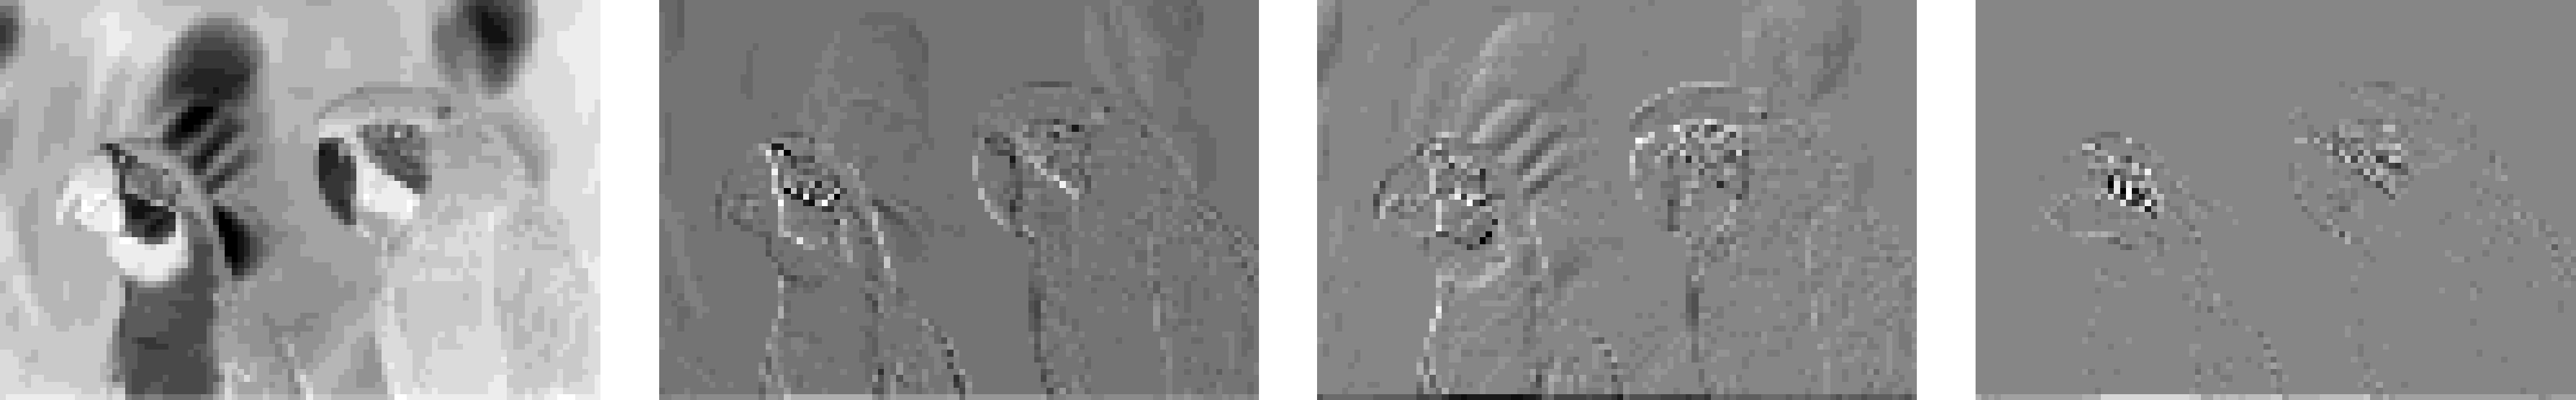
\includegraphics[width=.95\textwidth]{figures/kodim23_y_componets.pdf}
		\caption{}
		\label{fig: y componets}
	\end{subfigure}
	\begin{subfigure}{.455\textwidth}
		\centering
		\vspace{10pt}
		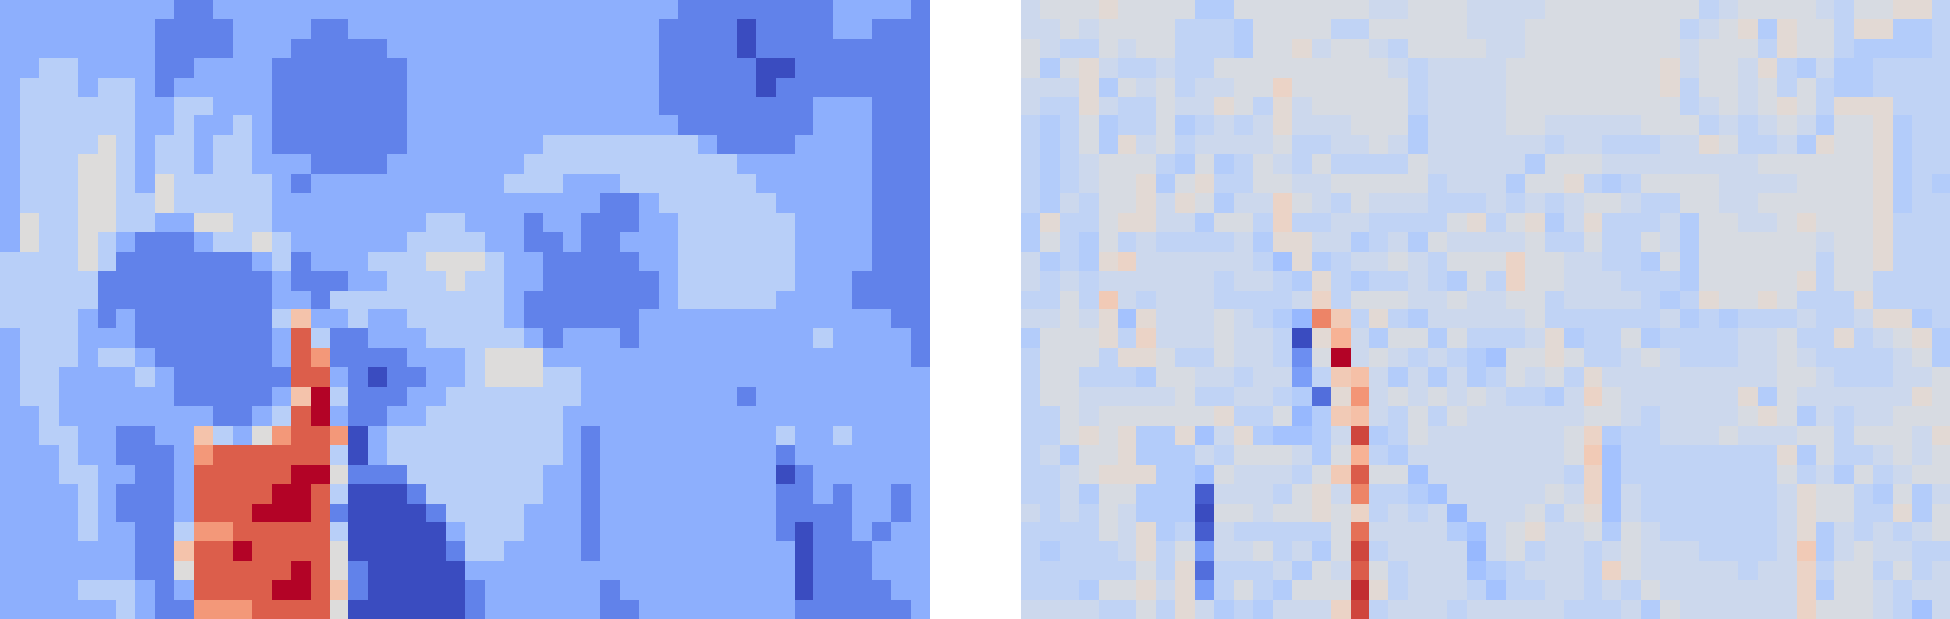
\includegraphics[width=.95\textwidth]{figures/kodim23_cb_componets.pdf}
		\caption{}
		\label{fig: cb componets}
	\end{subfigure}%
	\begin{subfigure}{.45\textwidth}
		\centering
		\vspace{10pt}
		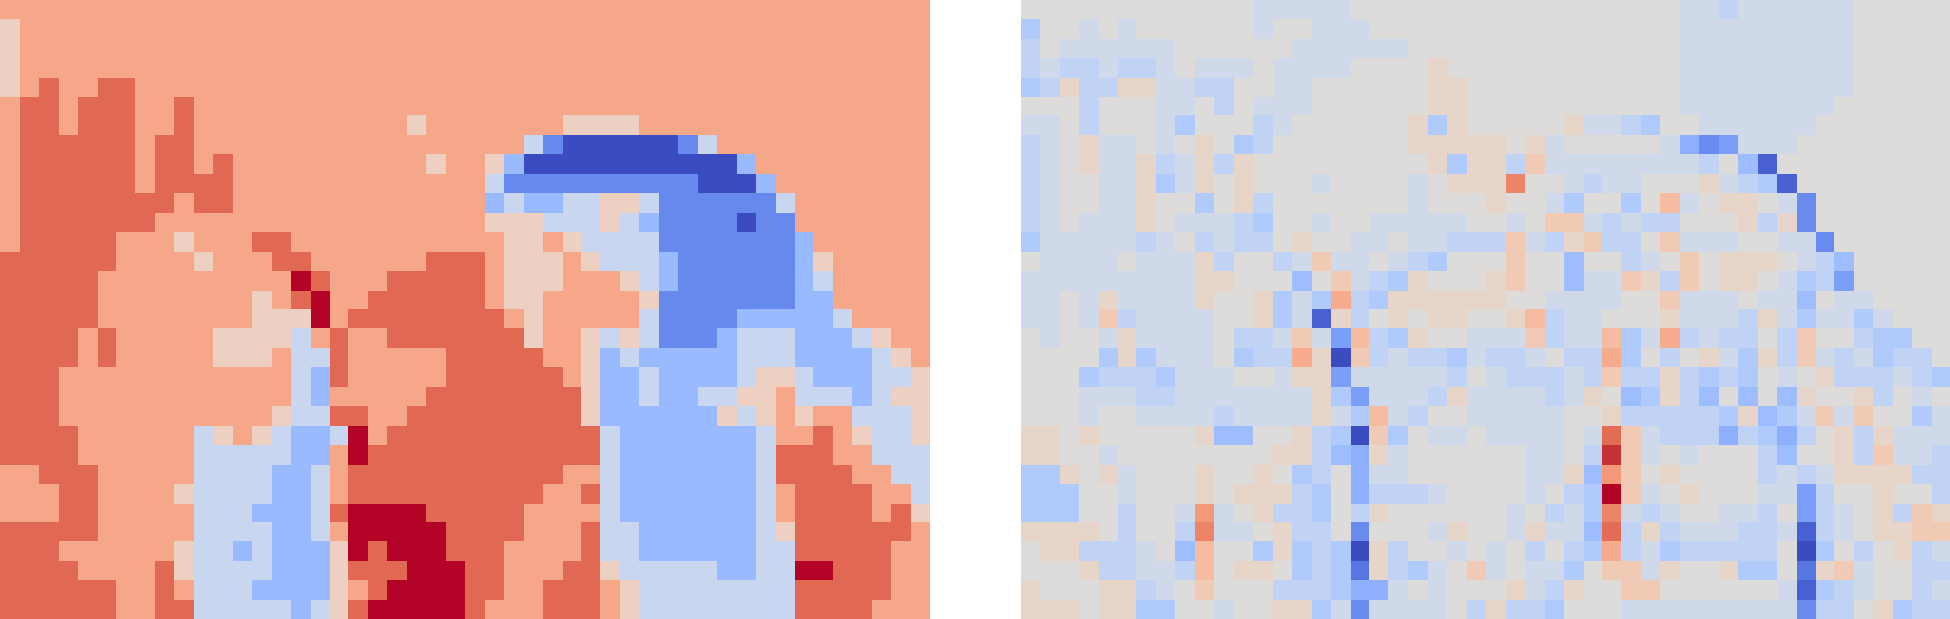
\includegraphics[width=.95\textwidth]{figures/kodim23_cr_componets.pdf}
		\caption{}
		\label{fig: cr componets}
	\end{subfigure}
	\caption{IMF components of the \texttt{kodim23} image from the Kodak dataset. Panels (a), (b), and (c) show the IMF components corresponding to luma (Y), blue-difference (Cb), and red-difference (Cr) chroma, respectively.}
	\label{fig:imf_components}
\end{figure}

The quantitative comparison is made in Fig.\ref{} on an image selected from the Kodak [] dataset. 
The images compressed by the considered compression methods are shown in different bits per pixel (bpp) values, a standard compression measure in the literature []. 
As can be seen, the IMF-based compression method is capable of maintaining quality compressed images in bpp values as low as $?$, outperforming JPEG and SVD-based methods which suffer from maintaining balanced colors as soon as bpp drops below $?$ and $?$, respectively. 
The artifacts in color are visible, e.g. by JPEG in bpp values starting $?$.


\subsection{Rate-Distortion Performance} \label{sec:rate_distortion_performance}
Peak signal-to-noise ratio (PSNR), as well as structural similarity index measure (SSIM) [], are reported versus bpp for the considered methods. 
The considered datasets are Clic [] and Kodak, consisting of respectively 32 and 24 colored images of various sizes.
For each image compressed by any of the considered methods, bpp, PSNR, and SSIM are calculated. 
Then, for each compression method, PSNR and SSIM values are interpolated linearly in the fixed bpp values in the range $(0.05, 0.5)$. 
In the following plots, the average performance over all images is reported, along with the standard deviation presented as shadows.
For the missing bpp values, the average is extrapolated quadratically and is shown by dashed lines.

In Fig.\ref{fig:compression_performance_kodak}, the compression performance on the Kodak dataset is reported. 
In this figure, the proposed IMF-based method outperforms the SVD-based method, which can be attributed to the quantization errors that SVD is prone to during encoding and decoding, deteriorating its performance in both criteria. In this view, the quantization-free property of IMF effectively guarantees higher performance in different bpp values.
It is also evident that the IMF-based method outperforms JPEG in low bpp values. The same performance regime can also be concluded for all the mentioned compression methods on the Clic dataset in Fig.\ref{fig:compression_performance_clic}.
\begin{figure}[t]
	\centering
	\begin{subfigure}{.5\textwidth}
		\centering
		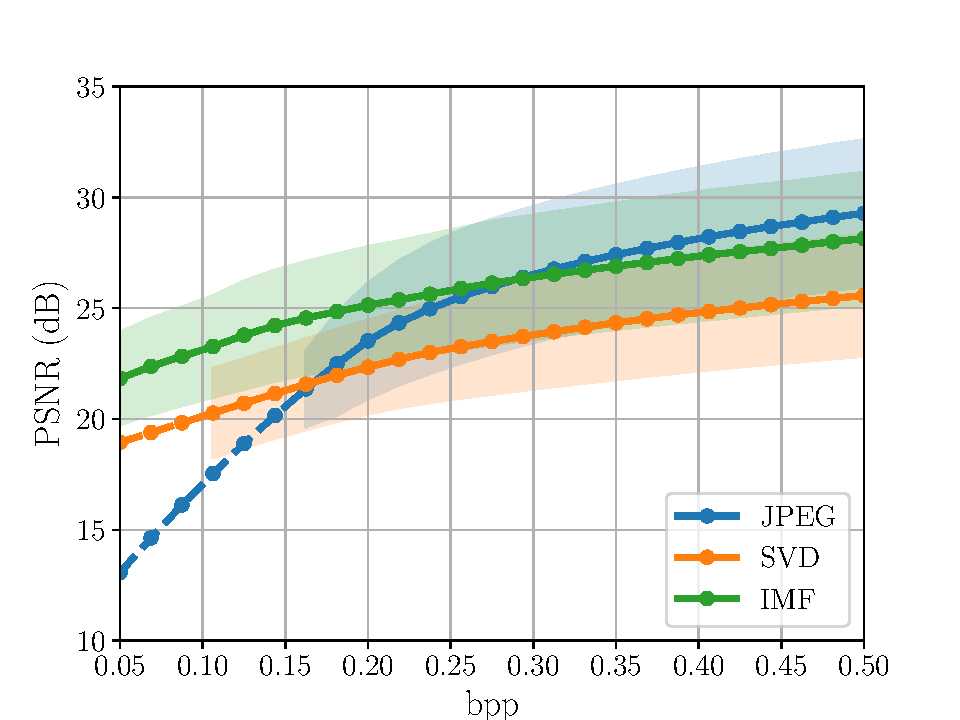
\includegraphics[width=.95\textwidth]{figures/comparison_kodak_psnr.pdf}
		\caption{}
		\label{fig: psnr-vs-bpp kodak}
	\end{subfigure}%
	\begin{subfigure}{.5\textwidth}
		\centering
		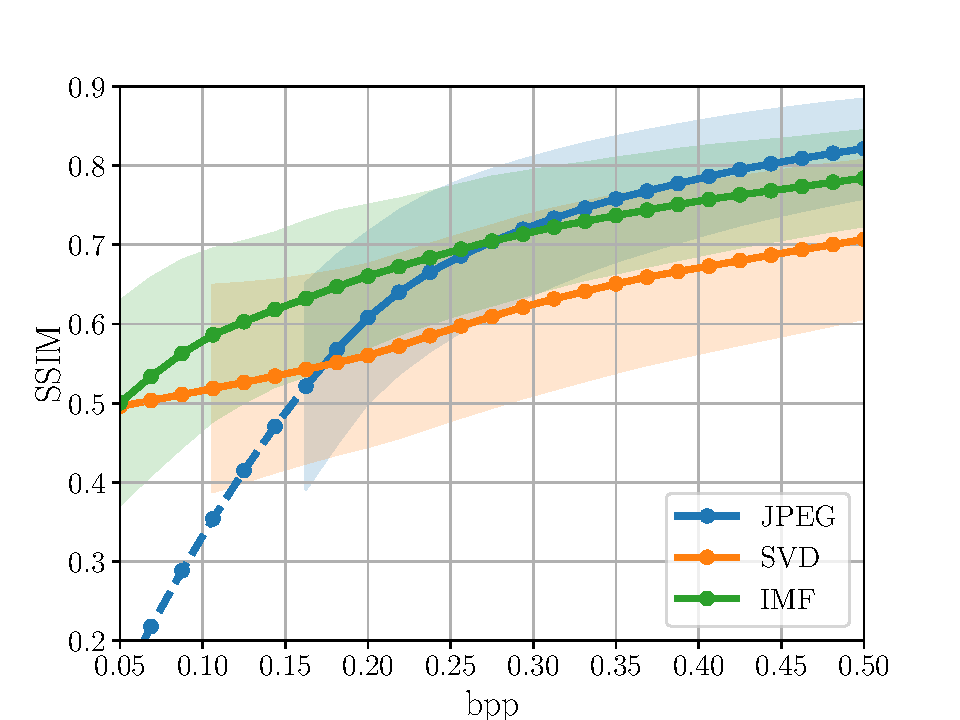
\includegraphics[width=.95\textwidth]{figures/comparison_kodak_ssim.pdf}
		\caption{}
		\label{fig: ssim-vs-bpp kodak}
	\end{subfigure}
	\caption{Rate-distortion performance on the Kodak dataset. In panels (a) and (b), the average PSNR and SSIM are plotted against bpp, respectively.}
	\label{fig:compression_performance_kodak}
\end{figure}

\begin{figure}[t]
	\centering
	\begin{subfigure}{.5\textwidth}
		\centering
		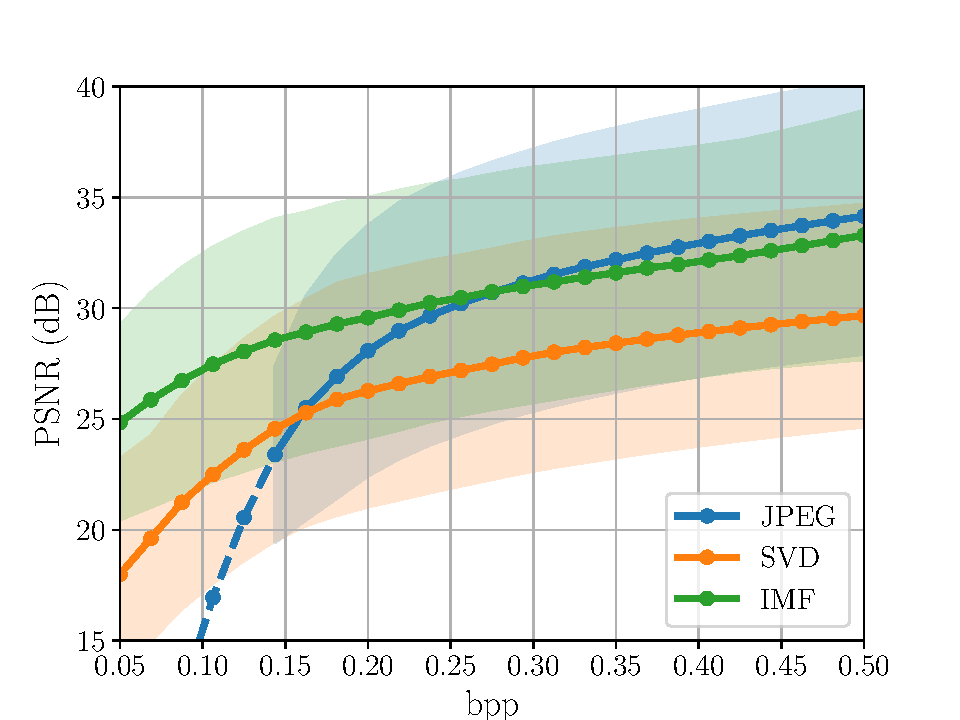
\includegraphics[width=.95\textwidth]{figures/comparison_clic_psnr.pdf}
		\caption{}
		\label{fig: psnr-vs-bpp clic}
	\end{subfigure}%
	\begin{subfigure}{.5\textwidth}
		\centering
		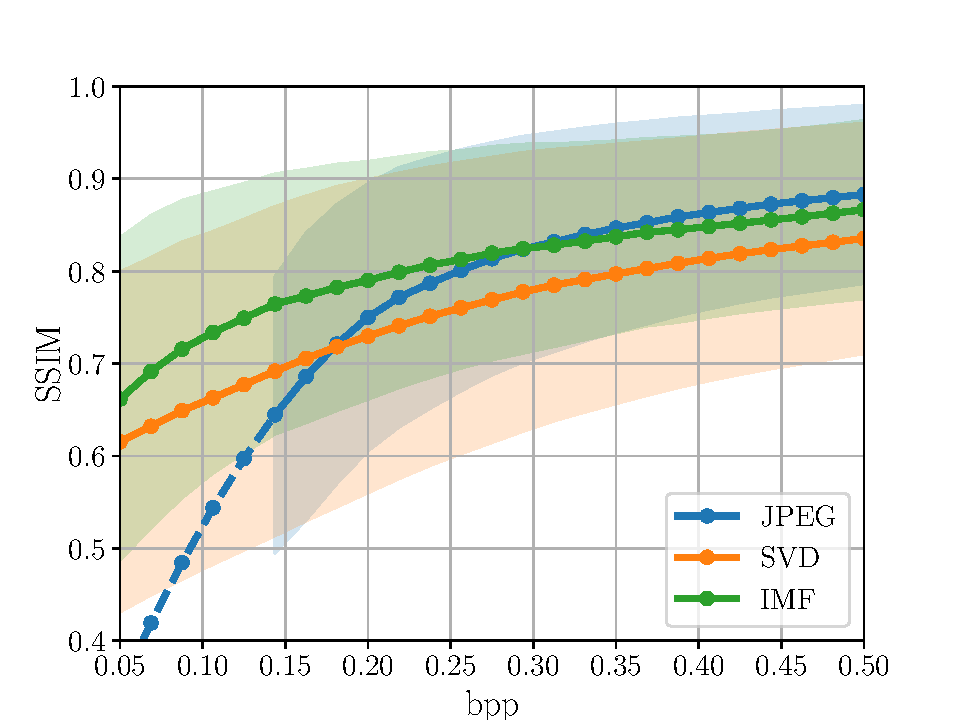
\includegraphics[width=.95\textwidth]{figures/comparison_clic_ssim.pdf}
		\caption{}
		\label{fig: ssim-vs-bpp clic}
	\end{subfigure}
	\caption{Rate-distortion performance on the CLIC dataset. In panels (a) and (b), the average PSNR and SSIM are plotted against bpp, respectively.}
	\label{fig:compression_performance_clic}
\end{figure}


\subsection{ImageNet Classification Performance} \label{sec: imagenet Classification Performance}
As another criterion, classification performance is investigated on the images compressed by the considered compression methods.
This criterion focuses on the higher-level information required for object recognition and classification embedded in each image.
Furthermore, it highlights the importance of image compression where various vision tasks such as classification are the main objective---rather than maintaining the perceived image quality---while keeping the requirement of resources such as memory, communication bandwidth, computation power, latency budget, etc. as limited as possible.
ImageNet [] validation set, consisting of 50000 $224 \times 224$ colored images in 1000 classes, is considered for this classification task done by a ResNet-50 classifier [], pre-trained on the original ImageNet dataset.
The classification performance comparison is made in Fig.\ref{fig:imagenet_classification}, showing the higher compression performance of IMF for classification, reaching top-1 accuracy of $70\%$ in bpp values as low as $0.2$. 

\begin{figure}[t]
	\centering
	\begin{subfigure}{.5\textwidth}
		\centering
				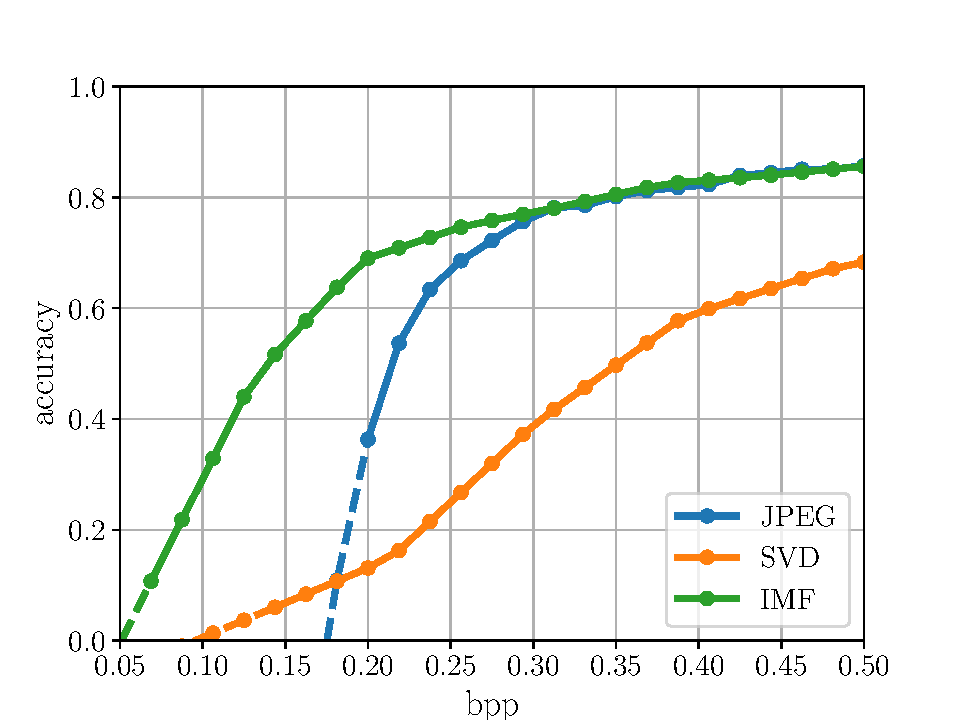
\includegraphics[width=.95\textwidth]{figures/classification_subset_performance_top1.pdf}
		\caption{}
		\label{fig: top1-vs-bpp imagenet}
	\end{subfigure}%
	\begin{subfigure}{.5\textwidth}
		\centering
				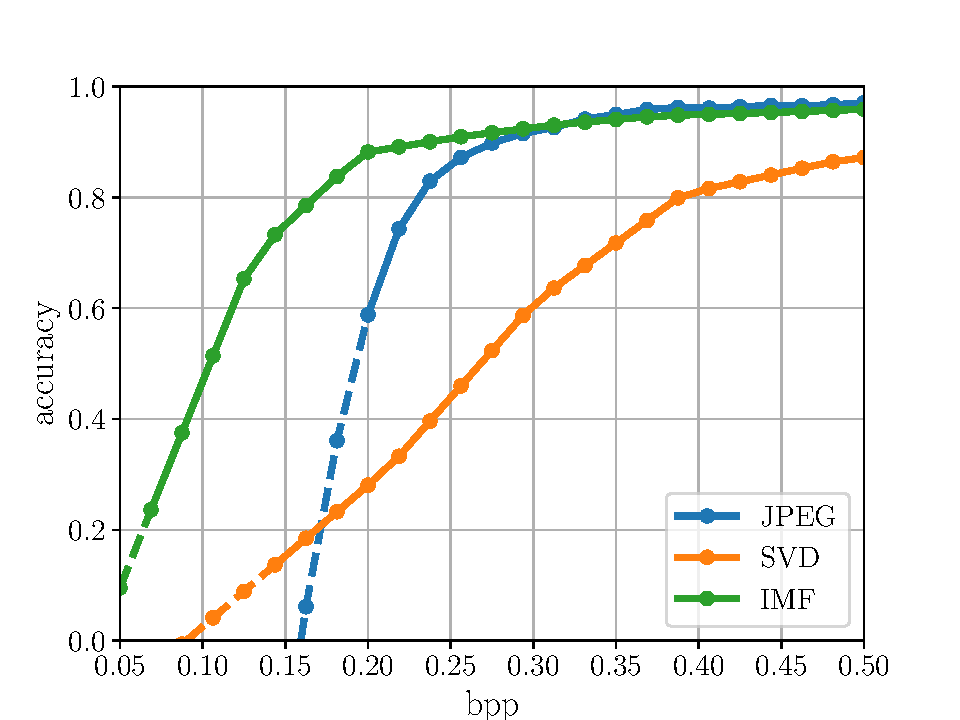
\includegraphics[width=.95\textwidth]{figures/classification_subset_performance_top5.pdf}
		\caption{}
		\label{fig: top5-vs-bpp imagenet}
	\end{subfigure}
	\caption{Impact of different compression methods on ImageNet classification accuracy. Panels (a) and (b) show the validation top-1 and top-5 accuracy plotted against bits per pixel (bpp), respectively. A ResNet-50 model pre-trained on the original ImageNet images is evaluated using validation images compressed by different methods.}
	\label{fig:imagenet_classification}
\end{figure}


\subsection{Ablation Studies} \label{sec: ablation studies}
In this section, ablation studies are performed, focusing on various hyper-parameters in the IMF-based compression method and their effect on the compression performance. 

\paragraph{Patchification.} 
In Fig.\ref{fig: patch ablation psnr-vs-bpp}, patchification effect with different patch sizes is investigated.
First, it can be concluded that patchification has a positive effect on performance. 
This performance boost is mainly due to the fact that in each patch (local) pattern variation is limited and hence IMF has more representation power to reconstruct the original pattern in each patch with fewer components. The performance on various datasets has shown that patches of size $8\times 8$ lead to the best performance. The same conclusion is evident for the Kodak dataset example presented in Fig.\ref{fig: patch ablation psnr-vs-bpp}.

\paragraph{Factor bounds.} 
As elaborated in Section \ref{sec: implementation details}, during the IMF optimization, IMF components are constrained into a bound $(-\alpha,\alpha-1)$. Fig.\ref{fig: bounds ablation psnr-vs-bpp} studies the compression performance versus different bounds. According to the results, the bound $(-16,15)$ leads to the best performance since the value distribution of IMF components lies mostly in this bound. Hence, dedicating fewer bits to represent this narrower bound compared to the other bounds results in higher compression rates without sacrificing performance. 

\paragraph{BCD iteration.}
The next parameter to study is the inner iteration number required in IMF BCD updates. 
According to the numerical results on various datasets, the objective value in the IMF optimization drops drastically after 2 iterations, while more iteration numbers have marginal improvement. 
This observation is shown for the Kodak dataset in Fig.\ref{fig: iteration ablation psnr-vs-bpp}.
This feature makes the IMF computationally efficient since with a limited number of iterations a high compression performance can be achieved.

\paragraph{Color space.}
The compression performance of IMF is studied with two color spaces, namely RGB and YCbCr, in Fig.\ref{fig: colorspace ablation psnr-vs-bpp}.
Although the compression performance remains unchanged in terms of PSNR, qualitative results reported in Fig.? indicate that YCbCr color space can maintain natural colors and brightness more effectively. Consistently, the JPEG method employs this color space as well.

\begin{figure}[t]
	\centering
	\begin{subfigure}{.5\textwidth}
		\centering
		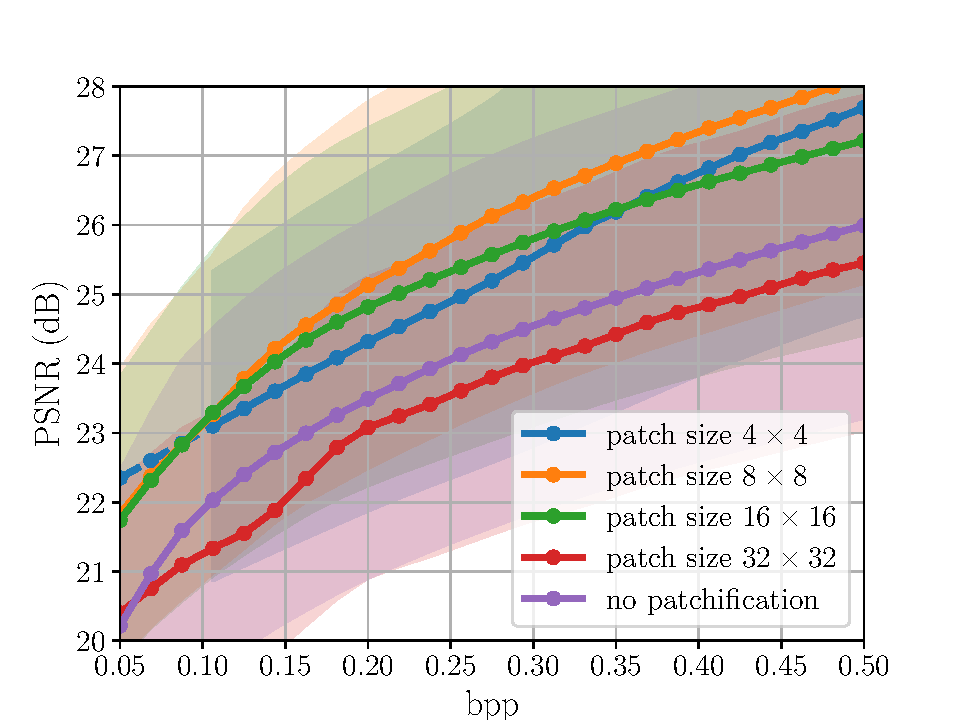
\includegraphics[width=.95\textwidth]{figures/ablation_patchsize_psnr.pdf}
		\caption{}
		\label{fig: patch ablation psnr-vs-bpp}
	\end{subfigure}%
	\begin{subfigure}{.5\textwidth}
		\centering
		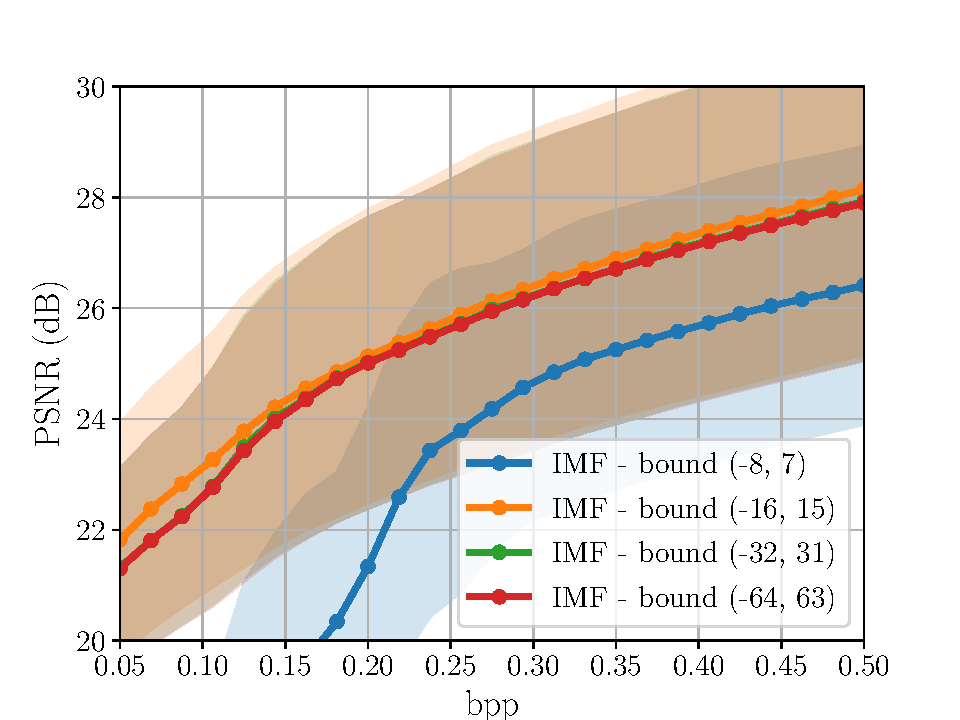
\includegraphics[width=.95\textwidth]{figures/ablation_bounds_psnr.pdf}
		\caption{}
		\label{fig: bounds ablation psnr-vs-bpp}
	\end{subfigure}
	
    \begin{subfigure}{.5\textwidth}
		\centering
		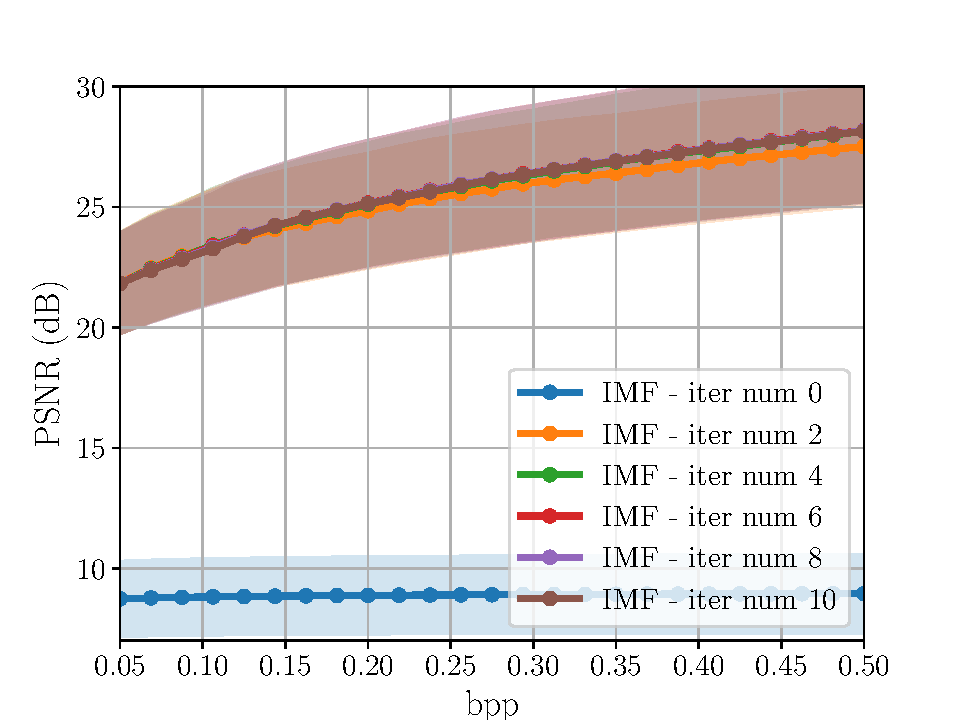
\includegraphics[width=.95\textwidth]{figures/ablation_iternum_psnr.pdf}
		\caption{}
		\label{fig: iteration ablation psnr-vs-bpp}
	\end{subfigure}%
	\begin{subfigure}{.5\textwidth}
		\centering
		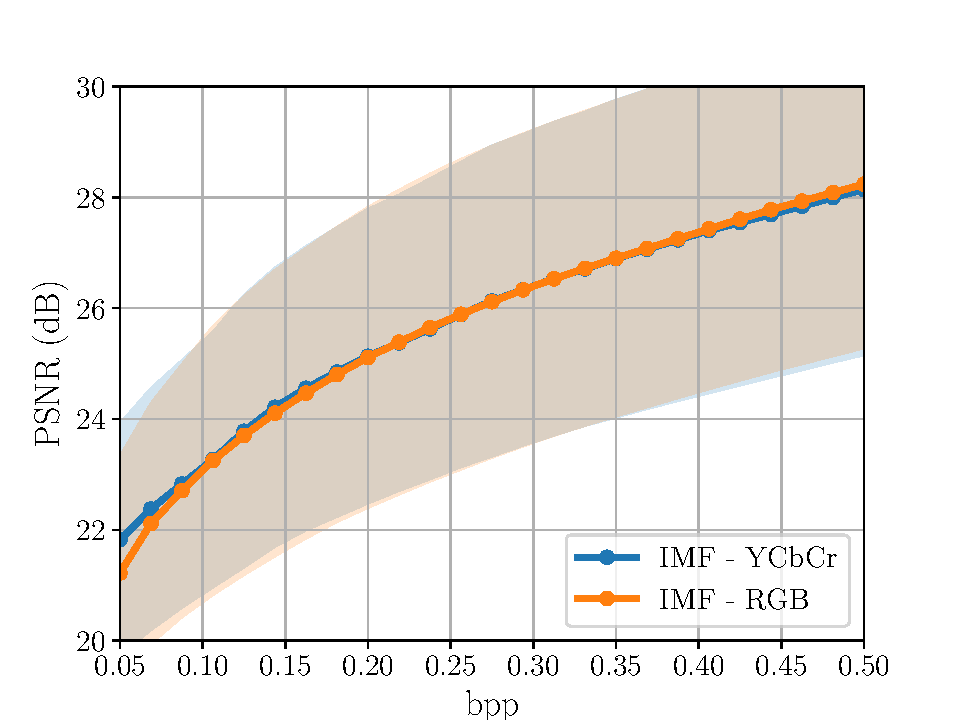
\includegraphics[width=.95\textwidth]{figures/ablation_colorspace_psnr.pdf}
		\caption{}
		\label{fig: colorspace ablation psnr-vs-bpp}
	\end{subfigure}
	\caption{Ablation experiments for the IMF compression method. In all cases, we plot PSNR as a function of bits per pixel (bpp) on the Kodak dataset. (a) Compares IMF compression performance without patchification and different patch sizes. (b) Compares IMF compression performance for different bound values of factor matrices. (c) Compares IMF compression performance for different numbers of BCD iterations. (d) Compares IMF compression performance between RGB and YCbCr color space transform.}
	\label{fig: ablation studies}
\end{figure}


